\chapter{Literature Survey}
\label{ch:literature-survey}

\quad This section will present an overview of the literature on routing protocols in \acrshort{manet}. An ad-hoc routing protocol is a convention or standard that regulates how nodes choose which method to route data between computing devices in a mobile ad-hoc network. According to the desired destination, ad-hoc network routing techniques are split into three types: unicast routing for a single destination, multicast routing for a group of destinations, and lastly broadcast routing for all targets in the network.

A comprehensive discussion of unicast routing protocols in \acrshort{manet}, particularly \acrshort{zhls} (our implemented approach), is given in sections 3.1, 3.2, and 3.3. In sections 3.3, 3.4, and 3.5, we will discuss multicast routing protocols, particularly \acrshort{odmrp} (our implemented approach).

\section{Unicast Routing in \acrshort{manets}}
\qquad The research interest in mobile ad-hoc networking grew rapidly in the 1990s. Because of the network's lack of infrastructure and dynamic nature, new networking methods must be adopted in order to ensure efficient end-to-end communication. This, combined with the numerous applications of these networks in various circumstances such as the battlefield and disaster recovery, has resulted in \acrshort{manets} routing being studied by a variety of organizations and institutes. The majority of \acrshort{manet} applications rely on unicast connectivity. The source mobile node transmits data packets to the destination in unicast mode. The destination address in the data packet is used by the dispatch node to search it up in the routing table when forwarding data packets\cite{unicast1}. \\

It's not easy to forward packets in a \acrshort{manet} with restricted resources (such as bandwidth restrictions, concealed terminals, and low battery power). To do this, a number of protocols have been developed. To decrease packet loss, communication overheads, and enhance data delivery ratio, various \acrshort{manet} unicast routing protocols have concentrated on attaining stability and dependability. Other unicast routing protocols have placed a premium on scalability to be capable of dealing with huge networks with minimum  computations. Other protocols placed an emphasis on data transmission speed and the ability to meet real-time constraints. To attain those objectives, many techniques have been developed. A comparative study of these Unicast routing techniques will be proposed in the next section.

\section{Comparative study of Unicasting}
The fundamental goal of ad-hoc routing protocols is to efficiently transmit data packets between nodes without relying on preset topologies or centralized management. Any unicast routing protocol must have the following characteristics: 
\begin{itemize}[itemsep=1pt, topsep=5pt]
    \item It should be assumed that routes are unidirectional.
    \item It should consider data security.
    \item It must be energy-and-power-efficient.
    \item It should be distributed in such a way as to enhance its dependability.
\end{itemize}  

Based on the previous properties, unicast routing techniques in \acrshort{manets} can be divided into three classes based on the time it takes for nodes to obtain a route to a destination. Those classes are reactive, proactive, and hybrid.

\subsection{Proactive routing protocols}
Proactive routing protocols, also known as table-driven routing protocols, require each node to maintain one or more tables containing up-to-date and consistent routing information for all other nodes in the network. these protocols learn the network's global topology by sharing information across network nodes. The nodes send out update messages every time the topology changes, and the knowledge about this change is disseminated across the network. Using this information, the shortest path can be computed from each source to any destination, but on the other side a lot of bandwidth is consumed\cite{unicast2}. In the following sections, some proactive routing protocols will be discussed.

\subsubsection{\acrfull{dsdv}}
The \acrfull{dsdv} is an extension of the well-known wired routing Distance Vector protocol. \acrshort{dsdv} addresses the primary problem associated with distance vector routing protocol in wired networks by utilizing destination sequence numbers, namely count-to-infinity. old routes and new routes are distinguished using sequence numbers originated at the destination, enabling the routing protocol to avoid route loops. multiple routes with the same sequence number are distinguished using the shortest route metric.\cite{abd2009performance}


\subsubsection{\acrfull{olsr}}
\acrfull{olsr} is an also extension and optimized variant of the well-known pure link-state routing protocol. It uses a multipoint relaying technique to efficiently transmit link-state packets. As the traditional link-state routing protocol, by sending link-state messages on a regular basis, each node keeps track of the network's topology. The optimization is mostly accomplished in two ways. First, during each route update, the size of the control packets for a specific node is reduced heavily by exchanging just a subset of links with the node's neighbors who are its multipoint relay selectors, rather than all links in the network. Each packet may be read and processed by any node not in the set, but it cannot be retransmitted. Second, it reduces control traffic flooding by employing just chosen nodes, known as multipoint relays, to distribute information in the network. Each node broadcasts a list of its one-hop neighbors to select these multipoint relaying nodes. A subset of these one-hop neighbors are chosen  from the list of nodes in the hello messages that covers all of its two-hop neighbors. Node A in Figure \ref{fig:multipoint relays} can choose MPR nodes from nodes B, C, K, and N. Because these nodes cover all nodes that are two hops apart.\cite{clausen2003optimized} \cite{clausen2003rfc3626}

\begin{figure}[!htb]
    \centering
    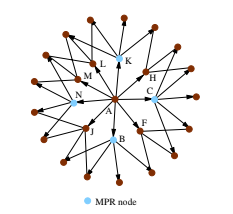
\includegraphics[scale=1]{images/olsr-mpr.png}
    \caption{Multipoint relays}
    \label{fig:multipoint relays}
\end{figure}

\subsubsection{\acrfull{fsr}}
\acrfull{fsr} is another optimized variant of the link-state routing protocol. It effectively reduces the amount of information and time it takes to keep network topology up to date. Link state updates are created and flooded across the network anytime a topology change is detected in the traditional link state routing method. However, in \acrshort{fsr}, nodes only communicate link status information on a periodic basis. By updating network information for local nodes at a higher frequency than for faraway nodes beyond the fisheye scope, \acrshort{fsr} lowers the size of update messages. As a result, \acrshort{fsr} is more scalable for huge networks. Figure \ref{fig:fsr} illustrate the \acrshort{fsr} hierarchical scopes.\cite{sathish2011comparative}

\begin{figure}[!htb]
    \centering
    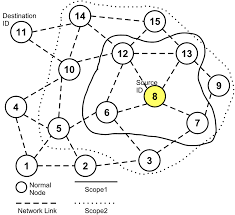
\includegraphics[scale=1]{images/fsr.png}
    \caption{Fisheye hierarchical scopes}
    \label{fig:fsr}
\end{figure}

\subsection{Reactive routing protocols}
On demand routing systems are also known as reactive protocols. By preserving route information for active routes, such protocol decreased the overheads of proactive protocol. It means that routing information is only necessary and stored when a node wishes to transmit a data packet to a specific destination. From the previous description, we can deduce that the main advantage for the reactive routing protocols over proactive routing protocol is to reduce the bandwidth waste. When route discovery is less frequent than data transmission, reactive routing systems function effectively\cite{unicast3}. Route discovery is generally accomplished by flooding the network with route request packets. When route discovery is less frequent than data transmission, reactive routing systems function effectively. 

\subsubsection{\acrfull{aodv}} 
With low control overhead and route acquisition delay, \acrfull{aodv} creates efficient routes on demand.
\acrshort{aodv} is essentially a hybrid of \acrfull{dsr} and \acrshort{dsdv} algorithms, using \acrshort{dsr}'s fundamental on-demand route discovery and maintenance mechanism as well as \acrshort{dsdv}'s usage of hop-by-hop routing sequence numbers to ensure loop-free routing. The source broadcasts a route request packet to determine a path from source to destination. The neighbors then broadcast the packet to their neighbors until it reaches an intermediary node with up-to-date route information about the destination or the destination itself. Because the route reply packet takes the same path as the route request packet, \acrshort{aodv} only needs symmetric connections. The nodes along the path insert the forward route into their tables as the route reply packet travels back to the source. Figure \ref{fig:aodv} illustrate the \acrshort{aodv} route discovery process. \cite{chakeres2004aodv} \cite{royer2000implementation}

\begin{figure}[!htb]
    \centering
    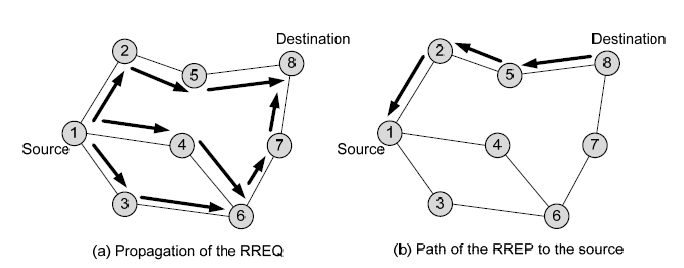
\includegraphics[scale=0.6]{images/aodv.png}
    \caption{\acrshort{aodv} route discovery}
    \label{fig:aodv}
\end{figure}

\subsubsection{\acrfull{dsr}}
\acrfull{dsr} offers a lot of advantages over routing protocols like \acrshort{aodv}, and it may perform better on small networks. \acrshort{dsr} has the benefit of allowing nodes to keep numerous routes in their route cache, allowing the node that wants to send a packet to some destination to check its route cache for a valid route before beginning route discovery, and if one is discovered, route discovery is not required. However, \acrshort{dsr} has a serious problem when dealing with huge networks, as its packets must carry the entire address (all hops in the path from source to destination). This indicates that this protocol will be ineffective on huge networks since the amount of overhead carried in each packet will grow as the network diameter grows, and it will consume a huge amount of bandwidth. Figure \ref{fig:dsr} illustrate how \acrshort{dsr} packets look like. \cite{usop2009performance} \cite{johnson2001dsr}

\begin{figure}[!htb]
    \centering
    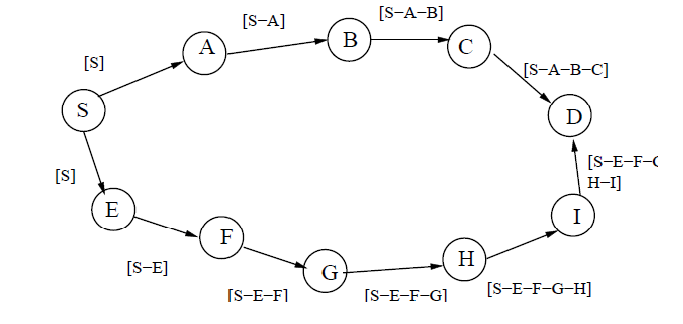
\includegraphics[scale=0.5]{images/dsr.png}
    \caption{\acrshort{dsr} packets}
    \label{fig:dsr}
\end{figure}

\subsection{Hybrid Routing Protocols}
Hybrid routing protocols are a new breed of protocol that is proactive as well as reactive. These protocols are intended to improve scalability by allowing nodes in proximity to collaborate to build a backbone that reduces route-finding overheads. The majority of this is accomplished by proactively maintaining routes to nearby nodes and finding routes to distant nodes using a route discovery strategy. The majority of hybrid protocols suggested to date are zone-based\cite{hybrid}, which implies that each node sees the network as a series of zones. In the next subsection, the \acrshort{zrp} routing protocol will be discussed, while in the next section the \acrshort{zhls} routing protocol will be discussed as our implemented approach.

\subsubsection{\acrfull{zrp}}
The nodes in \acrshort{zrp} each have a routing zone, which specifies a range (in hops) within which each node must maintain proactive network communication. As a result, routes are immediately available for nodes within the routing zone. Routes are determined on-demand for nodes outside the routing zone, and any on-demand routing protocol can be used to find a route to the needed destination. When compared to pure proactive protocols, this protocol has considerably reduced the amount of communication overhead. By allowing routes to be identified faster, it has also decreased the latency associated with pure reactive protocols like \acrshort{dsr}. This is because, in order to identify a route to a node outside the routing zone, the routing simply needs to go to a node on the required destination's borders (routing zone's edge). The drawback of \acrshort{zrp} is that it can operate as a pure proactive protocol for high values of routing zone, but as a reactive protocol for small values. \cite{beijar2002zone}

\subsubsection{\acrfull{zhls}}
\acrfull{zhls} split the whole network into zones that do not overlap. Each node in such a non-overlapping zone has a unique zone ID computed by GPS, and remember that each node in the whole network has a unique IP. The network's hierarchical structure (topology) is divided into two levels: node level topology and zone level topology, as shown in Figure \ref{fig:zhls}. Intrazone and interzone routing tables are created by each node using the flooded interzone and interzone LSR packets. When a node wants to transfer data packets to a node in another zone, the source node broadcasts a zone level “destination zone discovery (DZD)” request to all neighbor zones, which need much less overhead than reactive protocols' flooding techniques. After obtaining the destination zone, the data packets may be forwarded to the needed destination zone and subsequently to the required target node using the interzone then intrazone routing tables.\cite{joa1999peer} \cite{garg2012review} \cite{bansal2011performance} \cite{kamidate2007fault}

\begin{figure}[!htb]
    \centering
    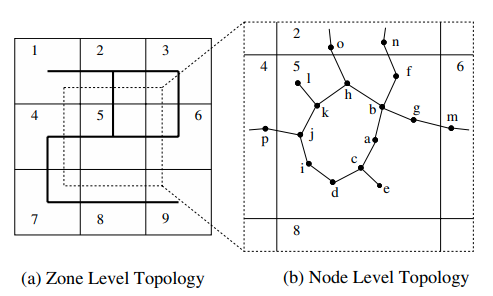
\includegraphics[scale=0.8]{images/zhls.png}
    \caption{\acrshort{zhls} network structure}
    \label{fig:zhls}
\end{figure}

\subsection{Overall Comparison of All Unicast
Routing Protocols }

Summary comparison of unicast routing protocols can be shown in Table \ref{tbl:unicast-comparison}
  
\begin{center}
\begin{table}[!htb]
\centering
\begin{tabular}{|>{\columncolor[HTML]{C0C0C0}}c |c|c|c|}
\hline
\textbf{
\begin{tabular}[c]{@{}c@{}}Routing Protocol\\ Parameter
\end{tabular}} &
  \cellcolor[HTML]{C0C0C0}\textbf{Proactive} &
  \cellcolor[HTML]{C0C0C0}\textbf{Reactive} &
  \cellcolor[HTML]{C0C0C0}\textbf{Hybrid} \\ \hline
\textbf{
\begin{tabular}[c]{@{}c@{}}Storage\\ Requirement
\end{tabular}} &
  High &
  Low &
  \begin{tabular}[c]{@{}c@{}}Depends on size\\ of each zone
  \end{tabular} \\ \hline
\textbf{\begin{tabular}[c]{@{}c@{}}Route\\ Availability\end{tabular}} &
  \begin{tabular}[c]{@{}c@{}}Always\\ available\end{tabular} &
  \begin{tabular}[c]{@{}c@{}}Computed as\\ per need\end{tabular} &
  \begin{tabular}[c]{@{}c@{}}Depends on\\ location of\\ destination\end{tabular} \\ \hline
\textbf{\begin{tabular}[c]{@{}c@{}}Periodic Route\\ Updates\end{tabular}} &
  Frequent &
  Sporadic &
  \begin{tabular}[c]{@{}c@{}}Used inside each\\ zone\end{tabular} \\ \hline
\textbf{Delay} &
  Low &
  High &
  \begin{tabular}[c]{@{}c@{}}Low for local\\ destinations and\\ high for interzone\end{tabular} \\ \hline
\textbf{Scalability} &
  100 nodes &
  \textgreater 100 nodes &
  \textgreater 1000 nodes \\ \hline
\textbf{Control Traffic} &
  High &
  Low &
  Medium \\ \hline
\textbf{\begin{tabular}[c]{@{}c@{}}Routing\\ Information\end{tabular}} &
  \begin{tabular}[c]{@{}c@{}}
  Stored in\\ table
  \end{tabular} &
  \begin{tabular}[c]{@{}c@{}}
  Does not\\ store
  \end{tabular} &
  \begin{tabular}[c]{@{}c@{}}
  Depends on\\ requirement
  \end{tabular} \\ \hline
\textbf{
\begin{tabular}[c]{@{}c@{}}
Routing\\ Philosophy
\end{tabular}} &
  Flat &
  Flat &
  Hierarchical \\ \hline
\end{tabular}
\caption{Summary Comparison of Unicast Routing Protocols}
\label{tbl:unicast-comparison}
\end{table}
\end{center}

\section{Implemented Unicast Routing: \acrshort{zhls}}
From the previous comparison, we can deduce that, in completely proactive protocols, nodes constantly attempt to maintain routes to all other nodes. This implies they monitor all topology changes in real-time. When there are a lot of nodes with a high mobility rate, this might be challenging, and it will consume a lot of bandwidth. On the other side, in completely reactive protocols, nodes only receive routing information on demand, and paths are only built when nodes have data for a specific destination. These techniques cut routing costs significantly, but their performance is variable since they are never prepared for disruptive occurrences.

We determined that a hybrid routing approach that combines aspects of both proactive and reactive routing techniques would best meet our application needs in light of these constraints. 

As stated above, Zone-Based Hierarchical Link State (\acrshort{zhls}) is one of the best hybrid routing protocols for many reasons. The management of \acrshort{zhls} nodes locations has been simplified. This is because the data transfer is not coordinated by a cluster head or a location manager. When compared to previous hybrid routing protocols, this implies there is no processing cost associated with cluster-head or Location Manager selection. This also implies that traffic bottlenecks and single points of failure may be avoided. When compared to pure reactive protocols like \acrshort{dsr} and \acrshort{aodv}, \acrshort{zhls} offers lower communication overheads. Consider the scenario when a route to a remote destination is needed (i.e., interzone routing). The source node broadcasts a zone-level location request to all other zones, resulting in much less overhead when compared to reactive protocols' flooding approach. Another advantage of \acrshort{zhls} is that the routing path may adapt to changing topologies because just the destination's node ID and zone ID are required for routing. As long as the destination does not relocate to another zone, no additional location searches are necessary.

The reasons we chose \acrshort{zhls} as a unicast routing method are summarized in the following points:

\begin{itemize}[itemsep=1pt, topsep=5pt]
    \item Simple location management as there is no cluster head or location manager node.
    \item It's ideal for tactical teams that are divided into groups and zones by nature.
    \item No traffic bottlenecks or single points of failure.
    \item Less memory requirements compared to proactive protocols.
    \item Lower control messages overhead using zone-level broadcasting compared to reactive protocols' flooding.
    \item Fewer computations when data is ready, so reduced battery usage as compared to reactive protocols.
    \item No location search is required as soon as the destination zone is known.
\end{itemize} 

There is always room for optimization. \acrshort{zhls} is one of the best unicast hybrid routing protocols but with some modifications, it can be better. The zone size is one of the most vexing aspects of any hybrid routing technology, particularly \acrshort{zhls}. The size of a zone has a significant impact on network performance. There is always a better zone size than another, depending on the application and the mobility of the nodes. So we thought, why not make the zone size a variable that the user may set depending on the application?
That was explained in details in system design section.

The second change was a technical one that affected the algorithm's implementation rather than its behavior. There will be nodes-level topology and zone-level topology, as well as intrazone and interzone forwarding tables, according to \acrshort{zhls}. Consider the scenario when a route to a remote destination is needed. the source node have to apply the shortest path algorithm on both zone-level topology and node-level topology and look at both interzone and intrazone tables depending on the destination zone. With adding one layer of abstraction to both nodes and zones, we managed to encapsulate both node IP and zone ID in one class. So now there's only one topology that contain both nodes and zones, there is also one forwarding table for both. That modifications imply fewer computations and less memory and battery consumption.

In comparison to the previous method, the third and final update significantly improves router performance and saves a significant amount of bandwidth. As previously stated, \acrshort{zhls} is a hybrid routing system, which implies it incorporates proactive routing approaches. The periodic changing of Interzone LSR control messages, which is used to convey zone information throughout the network, is one of these characteristics. The original technique required each node in each zone to flood this message, but just one node from each zone is enough because all nodes in the same zone will flood the same data. So, using some criteria, we were able to assign this work to only one node in each zone, greatly reducing control message overhead and improving system efficiency.


\section{Multicast Routing in \acrshort{manets}}
Multicast routing allows you to support group-oriented applications while using less bandwidth. Because of the growing demand for such applications, as well as the inherent characteristics of \acrshort{manets} such as lack of infrastructure and node mobility, secure multicast routing has become a critical yet difficult topic.

Multicast is an essential communication pattern that involves the sending of packets among a group of two or more hosts, and therefore is suitable for group-oriented computing. The use of multicasting in \acrshort{manets} has several benefits. For example, it can lower the cost of communication and increase the accuracy of the wireless channel, while transmitting numerous copies of the same data by exploiting the inherent broadcasting characteristics of wireless transmission. Instead of delivering data via multiple unicast connections, multicasting lowers channel capacity usage, reduces the cost of the sender and router's processing and energy, and communication latency. \cite{junhai2008research} \cite{junhai2009survey}

\subsection{Classification Of Multicast Routing Protocol}
Figure \ref{fig:mc-classification} demonstrates the dependency between the different and the main classification aspects for multicast routing protocol, including multicast topology, initialization approach, routing scheme, and maintenance approach.
\begin{figure}[!htb]
    \centering
    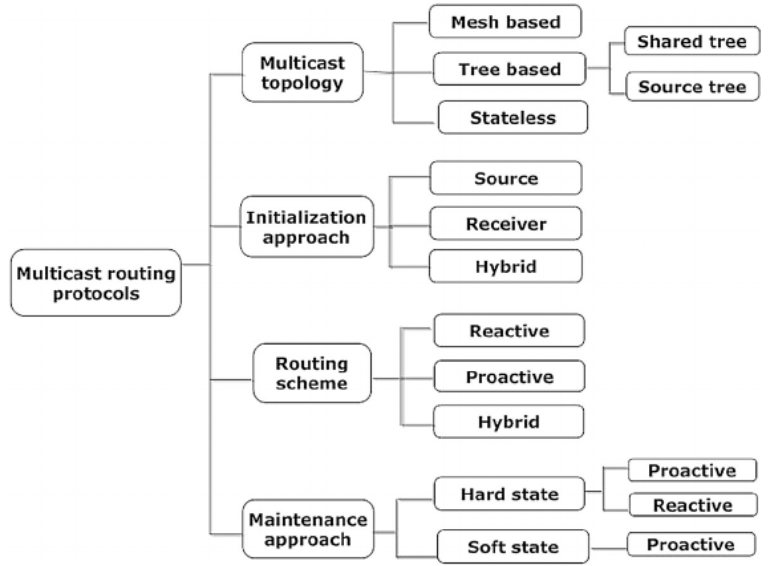
\includegraphics[scale=0.5]{images/mc-classification.png}
    \caption{classification of multicast routing protocols}
    \label{fig:mc-classification}
\end{figure}

\subsubsection{Multicast Topology}
Multicast topology has three approaches which are tree-based, mesh-based, and stateless approach. These three methods are described as follows:

\begin{enumerate}
\item Mesh-based approach

Mesh-based multicast protocols could have many routes between the same source and receiver pair. Current studies demonstrate that tree-based protocols are not always the best fit for multicast in a \acrshort{manet} when network topology changes often. In such an environment, mesh-based protocols tend to outperform tree-based approaches given the availability of different routes, which allows multicast datagram packets to be sent to the receivers even if connections fail. In this method, numerous routes are built in the whole network. These redundant routes are essential in link failure situation and give better packet delivery ratio 

\item Tree-based approach

Most systems for providing multicast in wired networks seem to be either source-tree-based or shared-tree-based. A unique route between source and receiver exists. This path and other paths are controlled by a general purpose node named core-node.

There are two main types of tree-based approach, which are described as follows:

\begin{itemize}
\item first is source-tree-based, whereby each source establishes a separated tree that includes the source node as the root node and then all receivers exist under this node.
\item second is shared-tree-based, in which one tree is created in the overall system, which contains all sources and receivers, so in this case, a core node controls the tree and behaves as a root to the tree.
\end{itemize}

\item Stateless approach

The stateless multicast approach, in which the source node explicitly specifies the list of targets in the packet header, is suggested to reduce the impact of such issues in tree-based and mesh-based approaches. Stateless multicast focuses on specific group multicast and expects the underlying routing protocol would take care of delivering the packet to appropriate destinations based on the addresses provided in the header.
\end{enumerate}

\subsubsection{Routing Initialization Approach}
Routing initialization is classified into three methods which are source-initiated, receiver-initiated, and hybrid approach. The three methods are described as follows:

\begin{enumerate}
\item Source-initiated approach

It is a method in which the multicast group creation and maintenance functions are handled by the source node. In order to start a new multicast group, the source node broadcasts a join query message all across the network, and any node wishing to join that multicast group responds by a join reply message. 

\item Receiver-initiated approach

It is a method in which the receiver node looks for a dedicated source inside the multicast group. The receiver node broadcasts a join query message across the network to enter a new multicast group, and thus the source node or core node responds by a join reply message containing the multicast group core route. 

\item Hybrid approach

The multicast group creation and maintenance functions are handled by either the source node or the receiver node in this method, which integrates specific characteristics from the source-initiated and receiver-initiated approaches. 
 
\end{enumerate}

\subsubsection{Routing Scheme}
Routing scheme is classified into three methods which are table-driven (proactive), on-demand (reactive), and hybrid approach. The three methods are described as follows:

\begin{enumerate}
\item Table-Driven Scheme (Proactive)

In a network using a proactive routing protocol, every node keeps one or more tables describing the complete network topology. These tables are frequently updated in order to keep up-to-date routing information of each node to any other node. To keep routing information up-to-date, topological information has to be transmitted between the nodes on a frequent basis, resulting in relatively significant overhead on the network. But on the other hand, routes will always be accessible on request. 

\item On-demand scheme (Reactive)

It attempts to build up routes on-demand, if a node wishes to start communication with another node to which it has no path, the routing protocol would seek to construct such a path. Reactive multicast routing protocol offers higher scalability than proactive multicast routing protocol. Unfortunately, while using reactive multicast routing protocol, source nodes may suffer from extra delay for path finding before they may send data packets. 

\item Hybrid scheme

It integrates the proactive and reactive methods in one strategy, in order to overcome the limits of both protocols and enhance their benefits. An example of a hybrid approach is zone routing protocol, which stores routing tables for a local zone, and creates routes on demand for targets outside this local neighborhood. It restricts the range of the local zone by describing a maximum hop number for the local zone. 
\end{enumerate}

\subsubsection{Multicast Maintenance Approaches}
Multicast maintenance is classified into two methods which are soft-state, and hard-state approaches. The two methods are described as follows:

\begin{enumerate}
\item Soft-state approach

This is a method in which broken link repair operation is started regularly by flooding the network with continuous control packets to seek alternative paths between source and destination. This method has the benefit of reliability and improved packet delivery ratios, but it creates considerable overhead over the network as it repeatedly floods the network with control packets. 

\item Hard-state approach

This is a method in which broken links maintenance procedure is created by two kinds, including reactive and proactive. In reactive methods, broken link recovery procedure is started only when a connection breaks. The second kind is proactive strategy, in which routes are reconfigured before a connection breaks, and this may be accomplished by using local prediction methods based on GPS or signal strength. 

\end{enumerate}

\section{Comparative study of Multicasting}
In this section we compare some commonly used multicast routing protocols and compare them and choose the best fit for our application, the comparative study done on the following protocols:
\begin{itemize}[itemsep=1pt, topsep=5pt]
    \item \acrfull{odmrp}
    \item Protocol for Unified Multicasting through Announcement (PUMA)
    \item Multicast Ad-hoc On demand Distance Vector Protocol (MAODV)
    \item Overlay Boruvka-based Ad-hoc Multicast Protocol (OBAMP)
    \item Application Layer Multicast Algorithm (ALMA)
    \item Enhanced version of ALMA (ALMA-H)
\end{itemize}

\subsection{Multicast routing protocols}
\begin{itemize}[itemsep=1pt, topsep=5pt]
\item \acrfull{odmrp}:

\acrshort{odmrp} \cite{ODMRP} is a reactive protocol which is mesh-based and source initiated protocol, it also maintains a mesh by following the soft-state approach.

\item Protocol for Unified Multicasting through Announcement (PUMA):

PUMA \cite{PUMA} is reactive protocol and distributed, it is mesh-based and receiver initiated protocol, PUMA’s all transmissions are broadcast and doesn’t depend on any unicast protocols.

\item Multicast Ad-hoc On demand Distance Vector Protocol (MAODV):

MAODV \cite{MAODV} is a reactive tree based protocol and hard-state, it uses a broadcast route discovery mechanism to discover the multicast routes on demand, it’s a multicast extension of the \acrshort{aodv} protocol.\cite{chow2008multiple}

\item Overlay Boruvka-based Ad-hoc Multicast Protocol (OBAMP):

OBAMP \cite{OBAMP} is a proactive mesh-first overlay multicast protocol, it is used to find the minimum spanning tree protocol which is a receiver initiated and soft-state approach.

\item Application Layer Multicast Algorithm (ALMA):

ALMA \cite{ALMA} is a proactive tree-based protocol, it is a receiver initiated protocol and soft-state approach, it is a flexible and highly adaptive overlay multicast protocol.

\item Enhanced version of ALMA (ALMA-H):

ALMA-H \cite{ALMA} is a proactive tree-based protocol, it is an enhanced version of ALMA for tree efficiency, it is a receiver driven and soft-state approach.


\end{itemize}

\subsection{Performance Evaluation Of Multicast Routing Protocols}

The performance evaluation criteria used to compare these protocols are Throughput, Reliability, End-to-End delay and Packet Delivery Ratio by increasing the numbers and speed of the nodes. \cite{multicast-survay}

\begin{enumerate}[itemsep=1pt, topsep=5pt]
    \item Throughput: the ratio between the number of data packets generated to the number of the data packets received.
    \item Reliability: the ratio of the successful end-to-end data delivery.
    \item End-to-end delay: the interval elapses between time of sending a packet and time of successfully delivering it.
    \item Packet Delivery Ratio: the ratio between the number of data packets delivered to the destination to the number of packets generated at the source.
\end{enumerate}

\subsubsection{Scenario is varying the number of nodes}
In this scenario the performance is measured for the four performance metrics by increasing the number of nodes from 20 to 80 with fixed speed of 0 m/s, the following graphs show the comparison between the performance of the six protocols.
\\
\\
Figure \ref{fig:nodes-vs} top left graph shows the simulation results of throughput in (Kbps) versus number of nodes.
\\
The results show that on increasing the number of nodes, \acrshort{odmrp} \cite{ODMRP} gives higher throughput than the other protocols that is because \acrshort{odmrp} deliver data packets in high rate as its operation is on-demand, on the other hand MAODV has the worst throughput as most of the nodes don’t participate in data transfer
\\
\\
Figure \ref{fig:nodes-vs} top right graph shows the simulation results of reliability versus the number of nodes where the number of senders is only one, so all protocols demonstrated high reliability.
\\
\acrshort{odmrp} and PUMA achieve the highest reliability as the number of nodes increases, the network becomes strongly connected and improves reliability.
\\
\\
Figure \ref{fig:nodes-vs} bottom left graph shows the end-to-end delay in (sec) versus the number of nodes.
\\
\acrshort{odmrp} shows the best delay performance than the other protocols because its route discovery mechanism is fast.
\\
\\
Figure \ref{fig:nodes-vs} bottom right graph shows the results of packet delivery ratio versus the number of nodes.
\\
\acrshort{odmrp} has a higher packet delivery ratio than the other protocols, PUMA and MAODV are pure on-demand protocols, however \acrshort{odmrp} is dynamic on-demand protocol.

\begin{figure}[!htbp]%
    \centering
    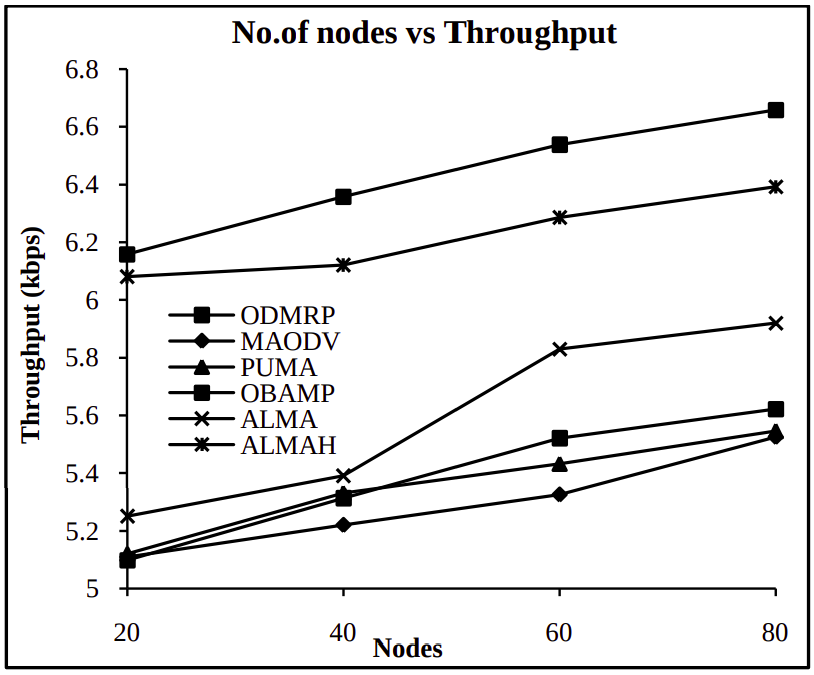
\includegraphics[width=7.8cm, height=7.8cm]{images/nodes-vs-throughput.png}
    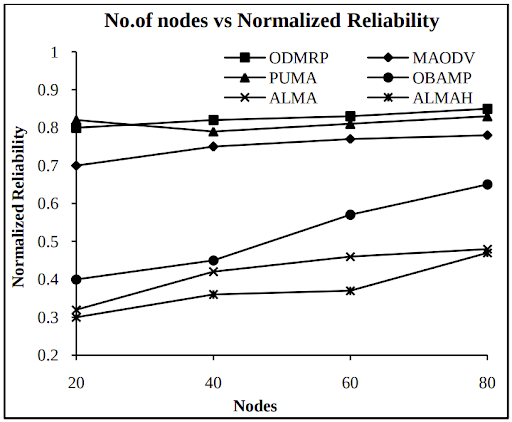
\includegraphics[width=7.8cm, height=7.8cm]{images/nodes-vs-reliability.png}
    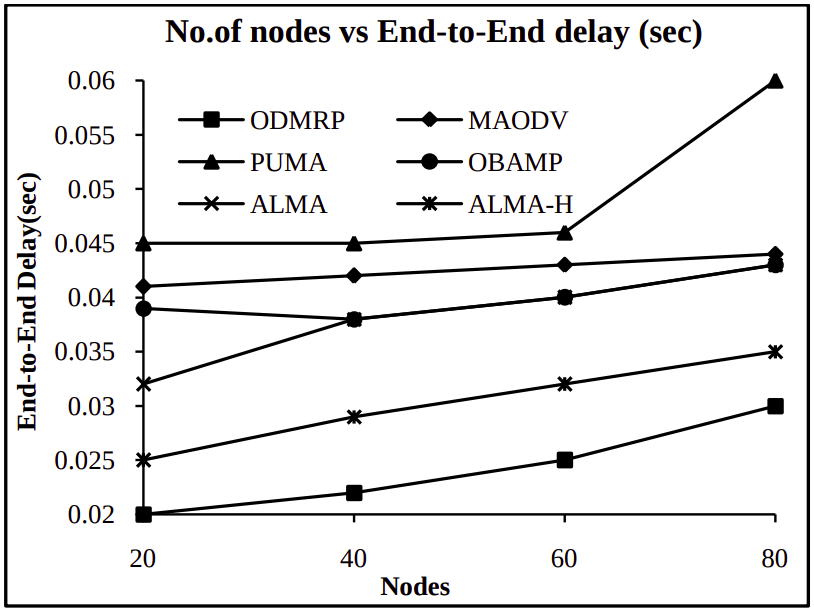
\includegraphics[width=7.8cm, height=7.8cm]{images/nodes-vs-e2edelay.png}
    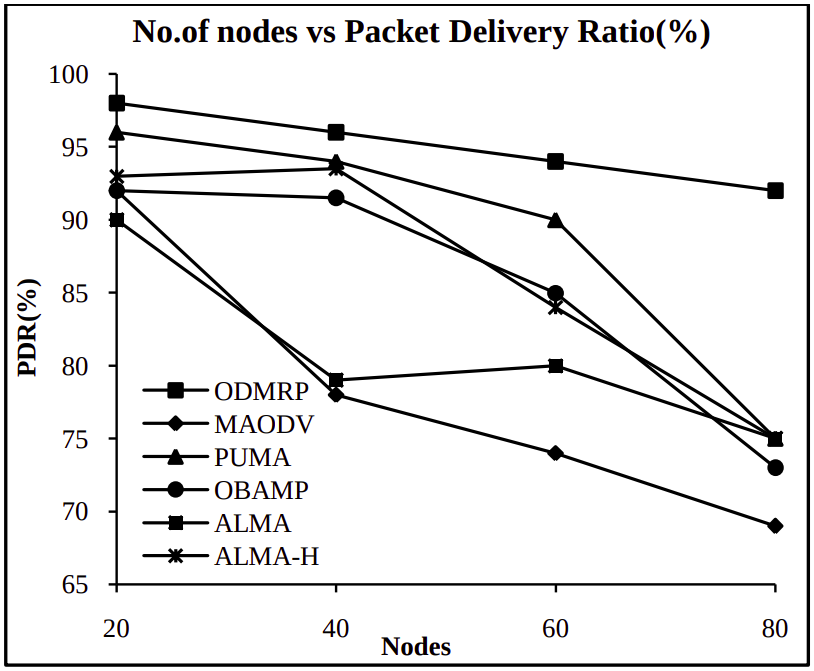
\includegraphics[width=7.8cm, height=7.8cm]{images/nodes-vs-pdr.png}
    \caption{Changing number of nodes vs reliability, throughput, delay and packet drop ratio}
    \label{fig:nodes-vs}
\end{figure}

\subsubsection{Varying the speed of nodes}

In this scenario the performance of the six protocols are measured for the four performance metrics by increasing the speed of nodes from 0 to 20 m/s with fixed number of nodes 80, the following graphs show the comparison between the performance of the six protocols.
\\
\\
Figure \ref{fig:mobility-vs} top left graph shows the simulation results of throughput versus the mobility speed in (m/s).
\\
We can see that the throughput decreases for all the six protocols as the mobility speed increases, and \acrshort{odmrp} has the best throughput as finding the route needs more routing traffic when speed increases. So less of the channel will be used to transfer data.
\\
\\
Figure \ref{fig:mobility-vs} top right graph shows the simulation results of reliability versus the mobility speed.
\\
We can see that by increasing the mobility speed \acrshort{odmrp} and ALMA-H have better reliability that the other protocols. This is because they have less transmission delay of messages.
\\
\\
Figure \ref{fig:mobility-vs} bottom left graph shows the simulation results of end-to-end delay versus mobility speed.
\\
When increasing the speed of the nodes, the topology changes frequently and then the probability of link breaking will increase. So additional route recovery process and route discovery process may be required. So as the speed increases, the end-to-end delay will also increase.
\\
\\
Figure \ref{fig:mobility-vs} bottom right graph shows the simulation results of packet delivery ratio versus mobility speed.
\\
The packet delivery ratio of all the protocols decreases when the speed increases, and \acrshort{odmrp} has better results than the other protocols.

\begin{figure}[!htbp]%
    \centering
    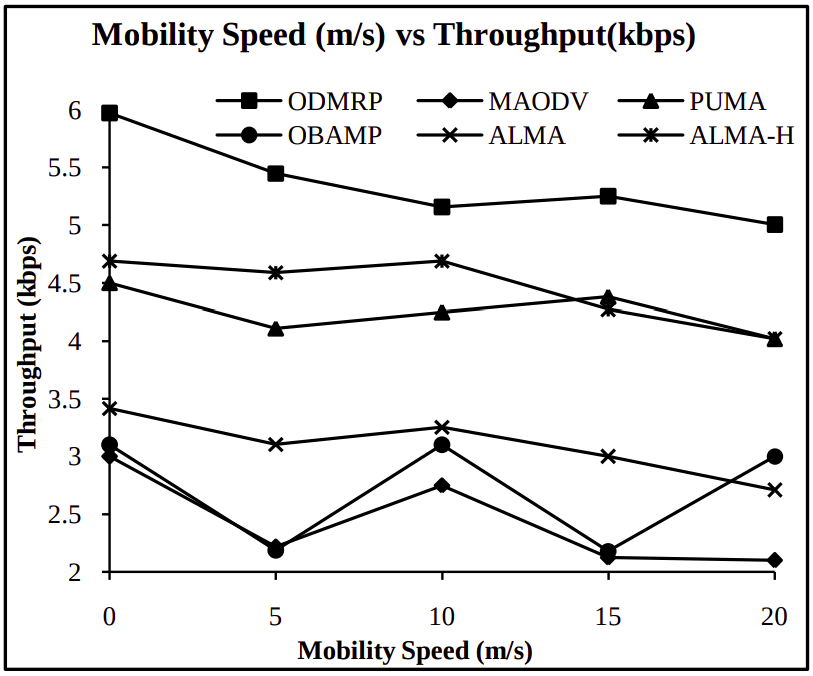
\includegraphics[width=7.8cm, height=7.8cm]{images/throughput-vs-mobility.png}
    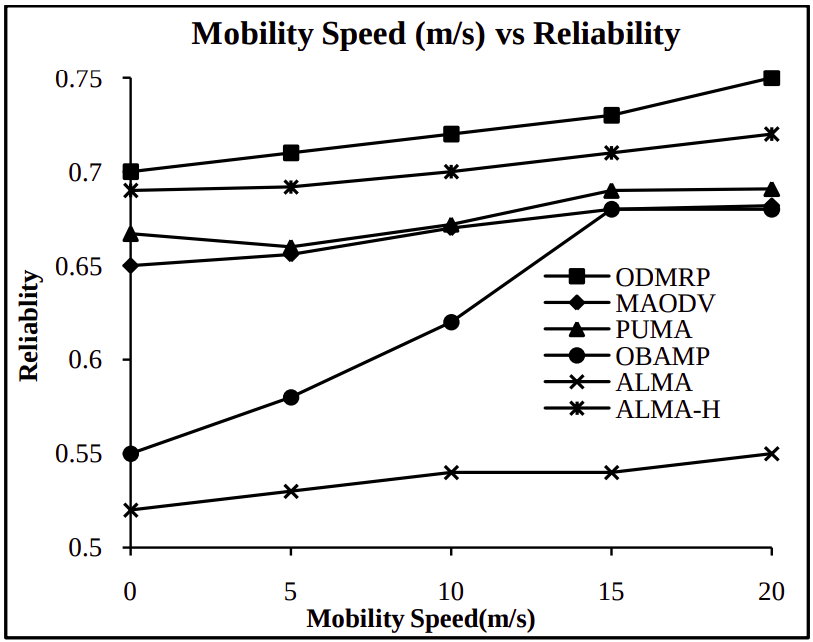
\includegraphics[width=7.8cm, height=7.8cm]{images/reliability-vs-mobility.png}
    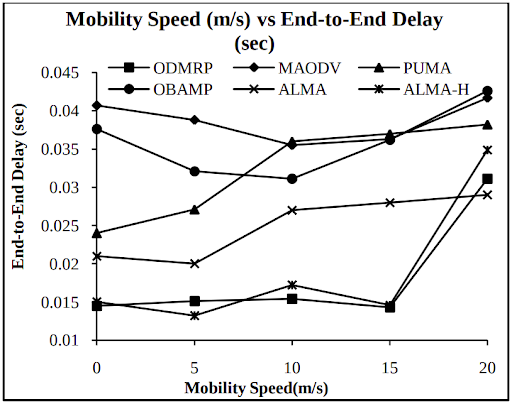
\includegraphics[width=7.8cm, height=7.8cm]{images/mobility-vs-e2edelay.png}
    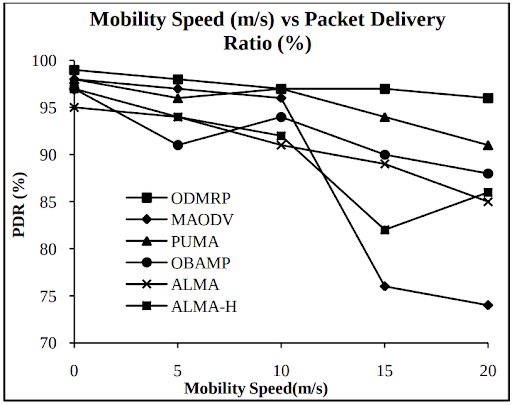
\includegraphics[width=7.8cm, height=7.8cm]{images/mobility-vs-pdr.png}
    \caption{Changing speed of nodes vs reliability, throughput, delay and packet drop ratio}
    \label{fig:mobility-vs}
\end{figure}

\section{Implemented Multicast Routing: \acrshort{odmrp}}
The Wireless Adaptive Mobility (WAM) Laboratory at the University of California, Los Angeles created the \acrfull{odmrp} \cite{ODMRP}, to reduce channel overhead and enhance scalability, \acrshort{odmrp} employs on-demand routing methods.
It constructs a forwarding mesh for each multicast group using the idea of a forwarding group, which is a collection of nodes responsible for passing multicast data.
The disadvantages of multicast trees in mobile wireless networks, such as inconsistent connectivity, traffic concentration, frequent tree reconfiguration, and non-shortest path in a shared tree, are addressed by maintaining and utilizing a mesh instead of a tree.
To keep multicast group members, a soft-state technique is used.
To quit the group, no specific control message is necessary.
We feel that \acrshort{odmrp} is more appealing in mobile wireless networks because of the reduced channel/storage overhead and the relaxed connection.
The advantages of \acrshort{odmrp} are highlighted by the features listed below.

\subsection{\acrshort{odmrp} Overview}
\acrshort{odmrp} is a mesh-based multicast scheme that employs a forwarding group idea to ensure that only a subset of nodes forwards multicast packets, rather than a traditional tree-based multicast scheme, It uses on-demand processes to create routes and manage multicast group membership dynamically.
\acrshort{odmrp} is ideally suited for ad hoc wireless networks with mobile hosts in which bandwidth is restricted, topology changes often and quickly, and power is limited.
\\
\\
The Query and Reply stages make up the \acrshort{odmrp}.
A packet Join Query is broadcast by source on a regular basis.
Every node in the network saves the upstream node address in the route database and rebroadcasts the packet to its neighbor nodes when it receives a non-duplicate Join Query packet via the reverse path technique.
When a multicast receiver receives a Join Query packet, it generates and transmits a Join Reply to its neighbors.
\\
Following the learned reverse path, this Join Reply packet is sent all the way back to the source, and the nodes on the reverse path become the forwarding group.
The following is how data is provided by the forwarding group nodes:
The source broadcasts data packets, while nodes in the forwarding group rebroadcast non-duplicate packets so that packets can be transmitted to recipients.
The forwarding group is a collection of nodes that are in charge of transmitting multicast data, thus establishing a mesh between all senders and receivers.
When a new node wishes to become a receiver in a multicast group, it waits for the next Join Query and replies with a Join Reply packet.
If a receiver becomes detached from the forwarding mesh owing to mobility, it must also wait for the next Join Query flooding.
\\
Without a local route recovery mechanism, \acrshort{odmrp}'s frequent route refresh and redundant forwarding maintain a high packet delivery ratio.
A soft-state technique is used in \acrshort{odmrp} to keep track of multicast group members; no explicit control messages are needed to join or exit the group.
A source node simply stops delivering a Join Query when it has no more packets to send.
If a receiver wishes to leave a multicast group, it does not answer to the multicast group's Join Query.
\\
If a forwarding node does not get the Join Reply after reaching a timeout that is a multiple of the refresh interval, it becomes a non-forwarder. 
\\
\\
After comparison to the previous routing protocols and other protocols using the four performance metrics: throughput, reliability, end-to-end delay and packet delivery ratio under two conditions: increasing the number of nodes and increasing the speed of the nodes. We found that In all cases, \acrshort{odmrp} outperforms the other multicast routing protocols, leading to the conclusion that \acrshort{odmrp} is effective and efficient in highly dynamic conditions and scalable to numerous multicast nodes, as for route discovery and maintenance, \acrshort{odmrp} uses periodic network-wide flooding. The purpose of this design is to guarantee robustness in the face of mobility and poor wireless connection propagation, and this feature would be very useful especially in rugged environments.

The reasons we chose \acrshort{odmrp} as our multicast routing protocol are summarized in the following points:

\begin{itemize}[itemsep=1pt, topsep=5pt]
\item The ability to route unicast traffic.

\item Low overhead in terms of channels and storage.

\item Use of the most recent shortest routes.

\item The ability to withstand host movement.

\item Reliable route and forwarding group development.

\item Wireless settings' broadcast nature is used.

\item Maintenance and exploitation of multiple redundant paths.

\item Scalability through the use of effective flooding.

\item The protocol's extensibility.

\item Limited power usage.
\end{itemize}

There is always room for optimization. \acrshort{odmrp} is one of the best multicast routing protocols but with some modifications as We did in broadcasting the join reply packets by using the filled tables to only sending the join reply packet to the upstream nodes, it also can be optimized further by other extendable versions of \acrshort{odmrp}:
\begin{itemize}[itemsep=1pt, topsep=5pt]
    \item E-\acrshort{odmrp} version of \acrshort{odmrp} with adaptive refresh. Rather than mobility prediction, receivers report connection breakages, which drives adaptation. A basic local recovery is easily incorporated with the adaptive refreshing method. In light load, EODMRP \cite{EODMRP} may have a slightly lower packet delivery ratio than \acrshort{odmrp}, but it may be better in high loads.
    \item RODMRP \cite{RODMRP} which seeks to be robust to network or node failures and to provide a continuous multicast service for live data streaming.
    \item It also could be extended to work with zones.
\end{itemize}

% @INPROCEEDINGS{MAODV,

%   author={Zhong, Mingyang and Fu, Yunqing and Jia, Xinqiang},

%   booktitle={2011 International Conference on E-Business and E-Government (ICEE)}, 

%   title={MAODV multicast routing protocol based on node mobility prediction}, 

%   year={2011},

%   volume={},

%   number={},

%   pages={1-4},

%   doi={10.1109/ICEBEG.2011.5881805}}
